
\section{Cold Spray}\label{sec:cold-spray}
Most engineering alloys, including stainless steel, aluminium and titanium, will undergo solid-state bonding when two atomically flat and clean surfaces are brought into contact, particularly in vacuum environments where surface contamination is minimal~\cite{merstallinger2009coldwelding}. 
This phenomenon is known as cold welding and occurs because the surface energy of the separated metal interfaces is higher than that of the bonded state, making direct bonding thermodynamically favourable~\cite{WagleBaker2015}. 

Designs typically aim to prevent this for space applications, but it is the core mechanism that underpins CSAM.\@ By accelerating metal powder particles to supersonic velocities and then impacting them upon the substrate, the particles cold weld to the surface forming a deposit. Seen in \autoref{fig:cs}, the particles plastically deform on impact, causing the disruption and removal of the oxide layer, and exposing a clean metal surfaces. 
\begin{figure}[htbp]
    \centering
    
    \begin{minipage}{0.45\textwidth}
        \centering
        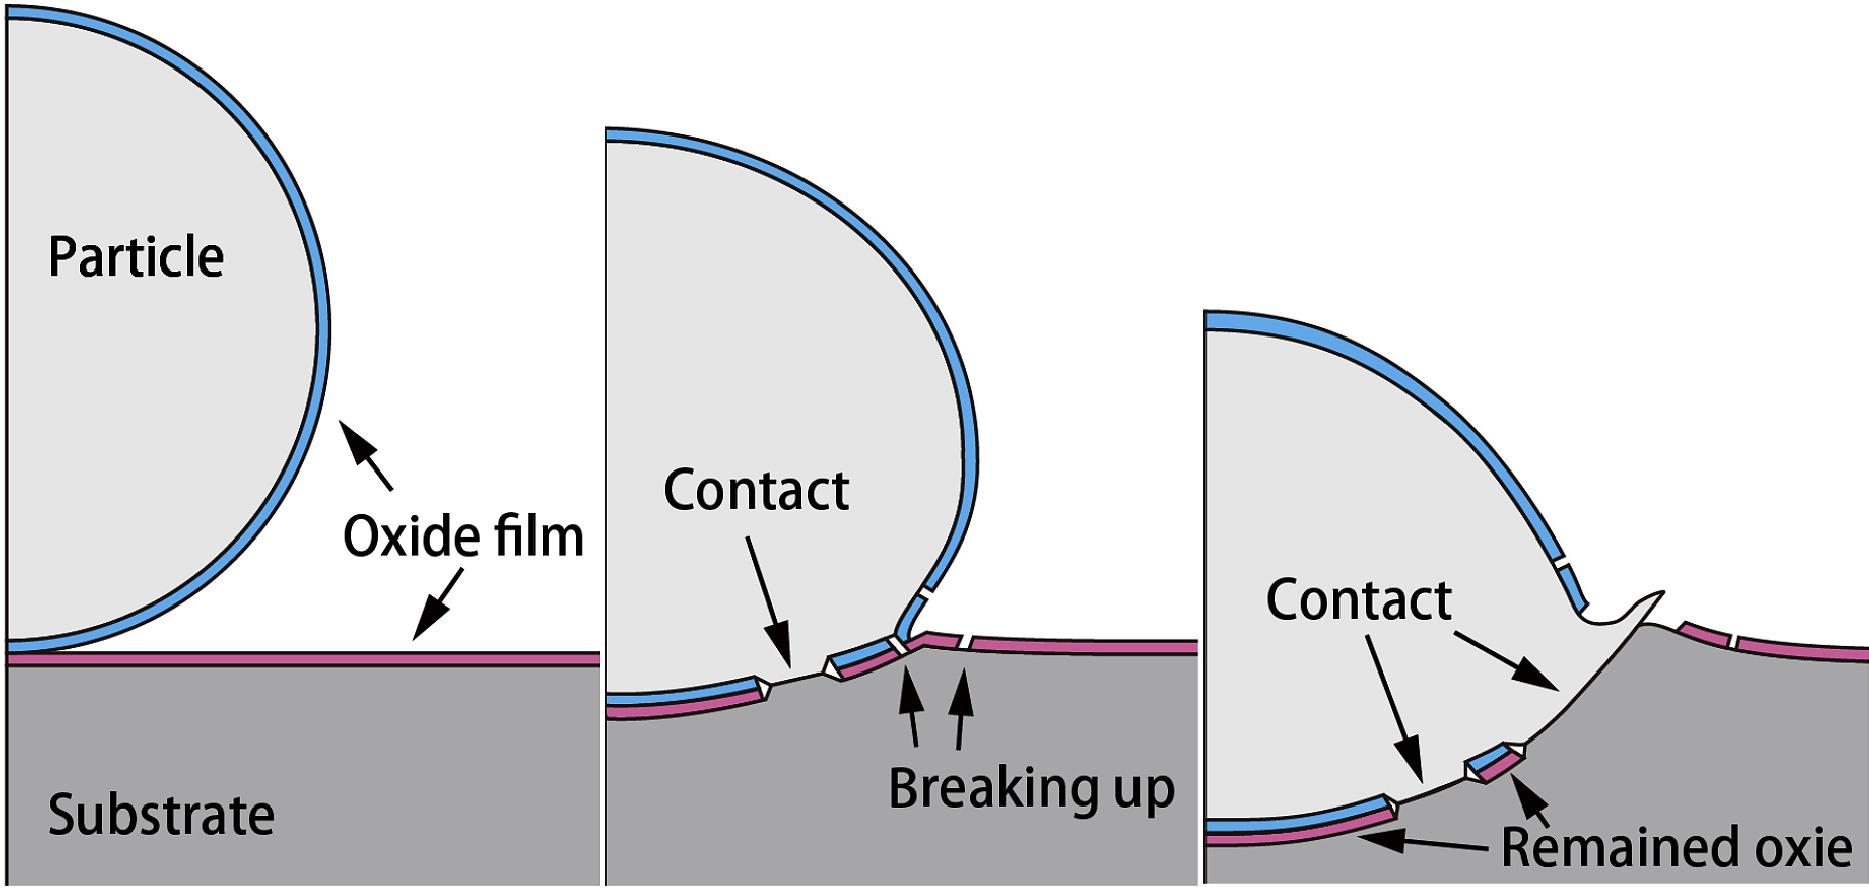
\includegraphics[width=\textwidth]{../report_assets/cs_bonding.png}
        \caption{Deformation and Bonding~\cite{ZHANG2024137157}}\label{fig:cs}
    \end{minipage}
    \hfill
    \begin{minipage}{0.45\textwidth}
        \centering
        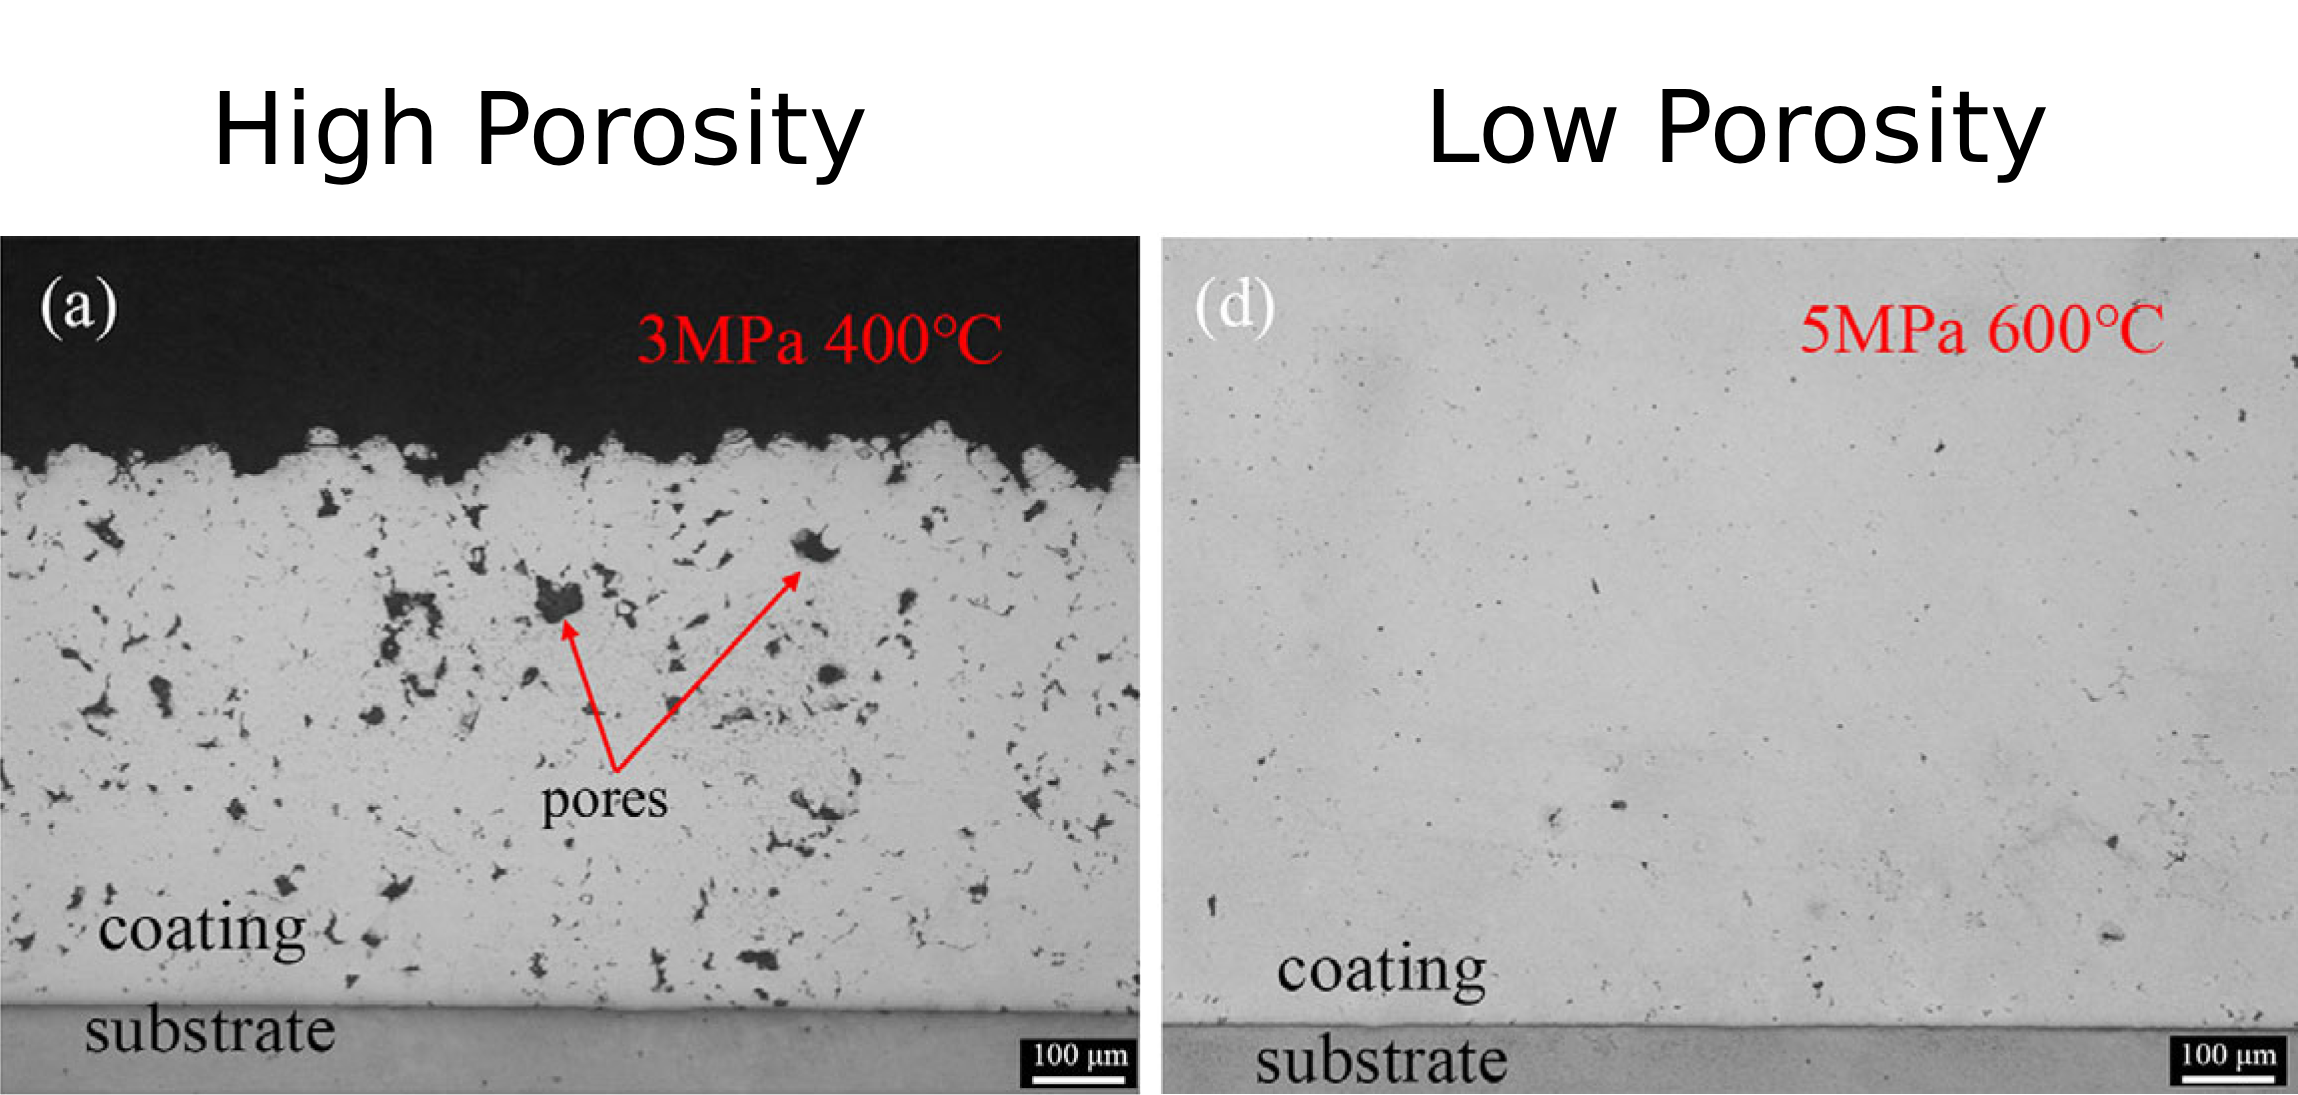
\includegraphics[width=\textwidth]{../report_assets/cs_porosity (1).png}
        \caption{Test Samples of CSAM~\cite{coatings13040738}}\label{fig:cs-porosity}
    \end{minipage}
    
\end{figure}
The removal of the oxide layer is thought to be because of adiabatic shear instability at the particle-substrate interface~\cite{assadi2016cold}, however, the precise mechanisms remain a topic of ongoing research and debate within the field~\cite{HASSANIGANGARAJ2018430}.

A unique advantage of CSAM is that it is a solid-state manufacturing process. Because the material never transitions through a liquid phase, thermal input remains low, preserving the original microstructure of both the powder and the underlying substrate. This minimises issues like residual thermal stresses, oxidation of the material and chemical composition inhomogeneity~\cite{ma16072765}. While solid-state manufacturing also tends to be better at reducing porosity, \autoref{fig:cs-porosity} shows that this can still be a problem depending on the parameters of the system. 

Arguably the most important parameter is the velocity of the particle impacting the surface. If this velocity is too low then bonding does not occur and if it is too high the powder roughens or erodes the substrate~\cite{Guo2022}. This velocity is dependent on the choice, pressure and temperature of accelerant gas and properties of the powder like mass flow rate, size, shape and hardness. All of these must be carefully chosen or controlled to produce high quality deposits.

\newpage

\section{Fluidised Powder Bed Phenomenon}\label{sec:background-powder-beds}
Given that fluidisation underlies the design architecture presented later, the physics behind a generic fluidised powder bed are outlined in this section. The powder in these systems exhibit distinctive fluid-mechanical behavior once a sufficient gas flow is passed upward through the granular solid~\cite{KuniiLevenspiel1977}. Shown in \autoref{fig:fluidisation}, as the gas velocity increases from zero, the powder initially remains fixed with the gas passing through void spaces, known as a fixed bed regime. At a critical threshold, the minimum fluidisation velocity, the drag force exerted by the gas equals the effective weight of the particles, causing the bed to loosen and particles to become suspended.
\begin{figure}[htbp]
    \centering
    
    \begin{minipage}{0.63\textwidth}
        \centering
        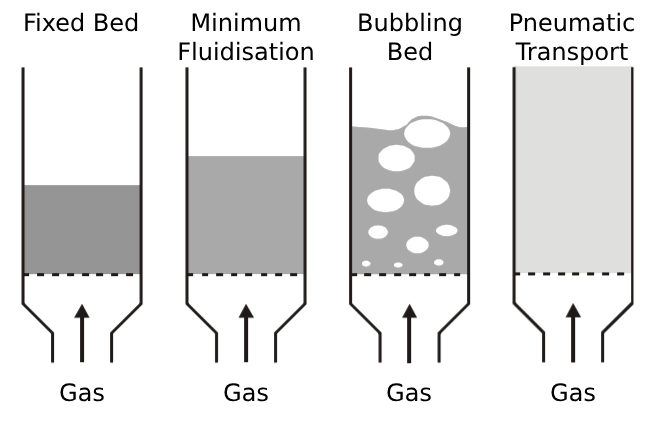
\includegraphics[width=\textwidth]{../report_assets/fluidisation_phases_diagram.png}
        \caption{Different Phases of Fluidisation~\cite{klaren2021fluidization}}
    \end{minipage}
    
\end{figure}\label{fig:fluidisation}
At this threshold, the pressure drop across the bed reaches a plateau, approximately matching the weight of the solid particles per unit area, and the powder itself begins to swell in volume, known as bed expansion. The expansion corresponds to an increase in average porosity as particles are pushed further apart in the fluid-like suspension. With further increases in gas flow, the fluidised bed exhibits bubbling behavior. In gas-fluidised systems at ambient pressure, any gas in excess of that needed to just fluidise the bed passes through in the form of buoyant gas voids or bubbles~\cite{SHENG2022137168}.

At the particle scale, motion results from the interplay of buoyancy, drag, and either cohesion or gravitational forces depending on the size. For smaller particles with a diameter of $20\,\mu\mathrm{m}$, it was found numerically that they are most influenced by cohesion and particles of $75\,\mu\mathrm{m}$ by gravity~\cite{SUN201785}.  This means the equilibrium for heavier particles may break down in microgravity, making space-based applications particularly challenging to predict or analyse. While the author is aware that research around the topic of particle dynamics under microgravity conditions exists, no research on the behaviour of fluidised powder beds or how to model this in a low gravity regime was found. Therefore, the effects of microgravity on the fluidisation physics has been deemed out of the scope of the project and disregarded, assuming that fluidisation will still occur due to cohesion.

\newpage

\section{Fluidised Powder Feed System Design Evolution}\label{sec:fluidised-powder-feed-systems}
The final architecture chosen in \autoref{sec:system_architecture} borrows heavily from research into metallic powder fed engines. As both systems have strict mass flow rate control and miniaturaisation requirements, the analysis can be used to reach a more elegant design. These systems have undergone multiple revisions to improve performance and this timeline is outlined to better explain the architectures behaviour.

A commonly cited first implementation of a fluidising powder feed system consists of a cylindrical tank with a piston to constrain the powder to the outlet~\cite{LI2021712}. As this paper is no longer in the public domain, exact parameters are unknown but developments from this design can be split into 3 phases.

The first of these improvements is the use of a gas-actuated piston instead of one driven by a motor~\cite{TANG2023118406}, examples of each are provided in \autoref{fig:actuation-piston}. The additional mass of an electric motor and the electrical systems to support it can be forgone by rerouting the high pressure line already close to the tank.
\begin{figure}[htbp]
    \centering
    
    \begin{minipage}{0.35\textwidth}
        \centering
        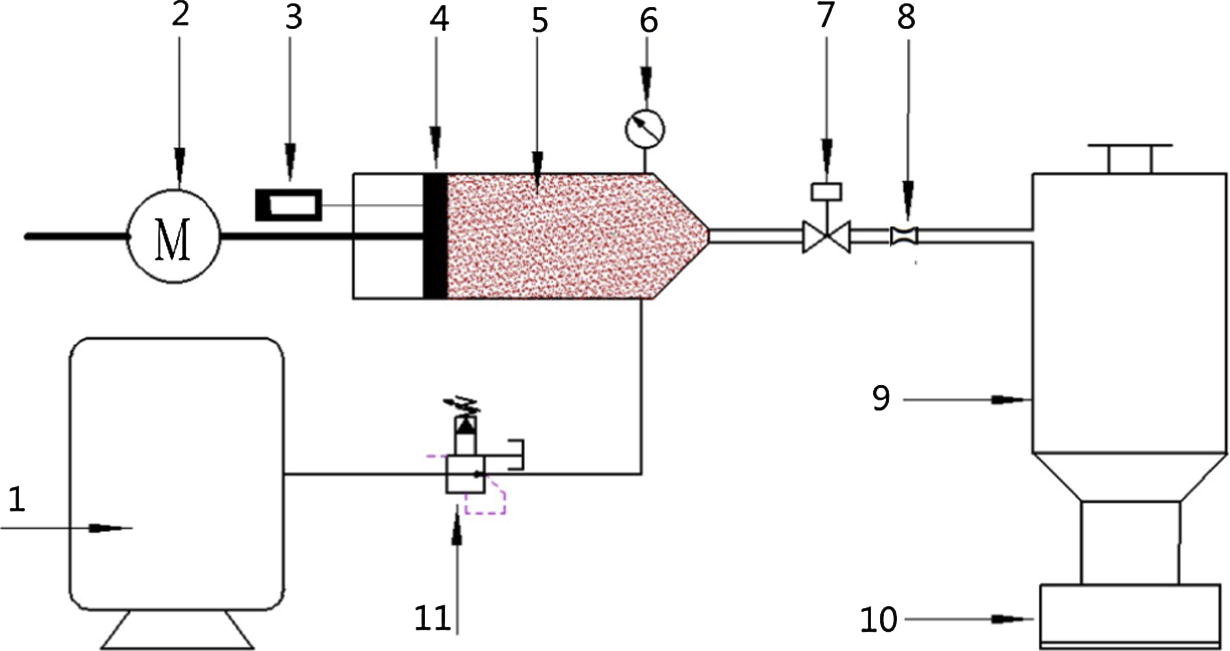
\includegraphics[width=\textwidth]{../report_assets/motor_driven.png}
        \caption*{Motor Driven Piston~\cite{SUN201630}}
    \end{minipage}
    \hfill
    \begin{minipage}{0.55\textwidth}
        \centering
        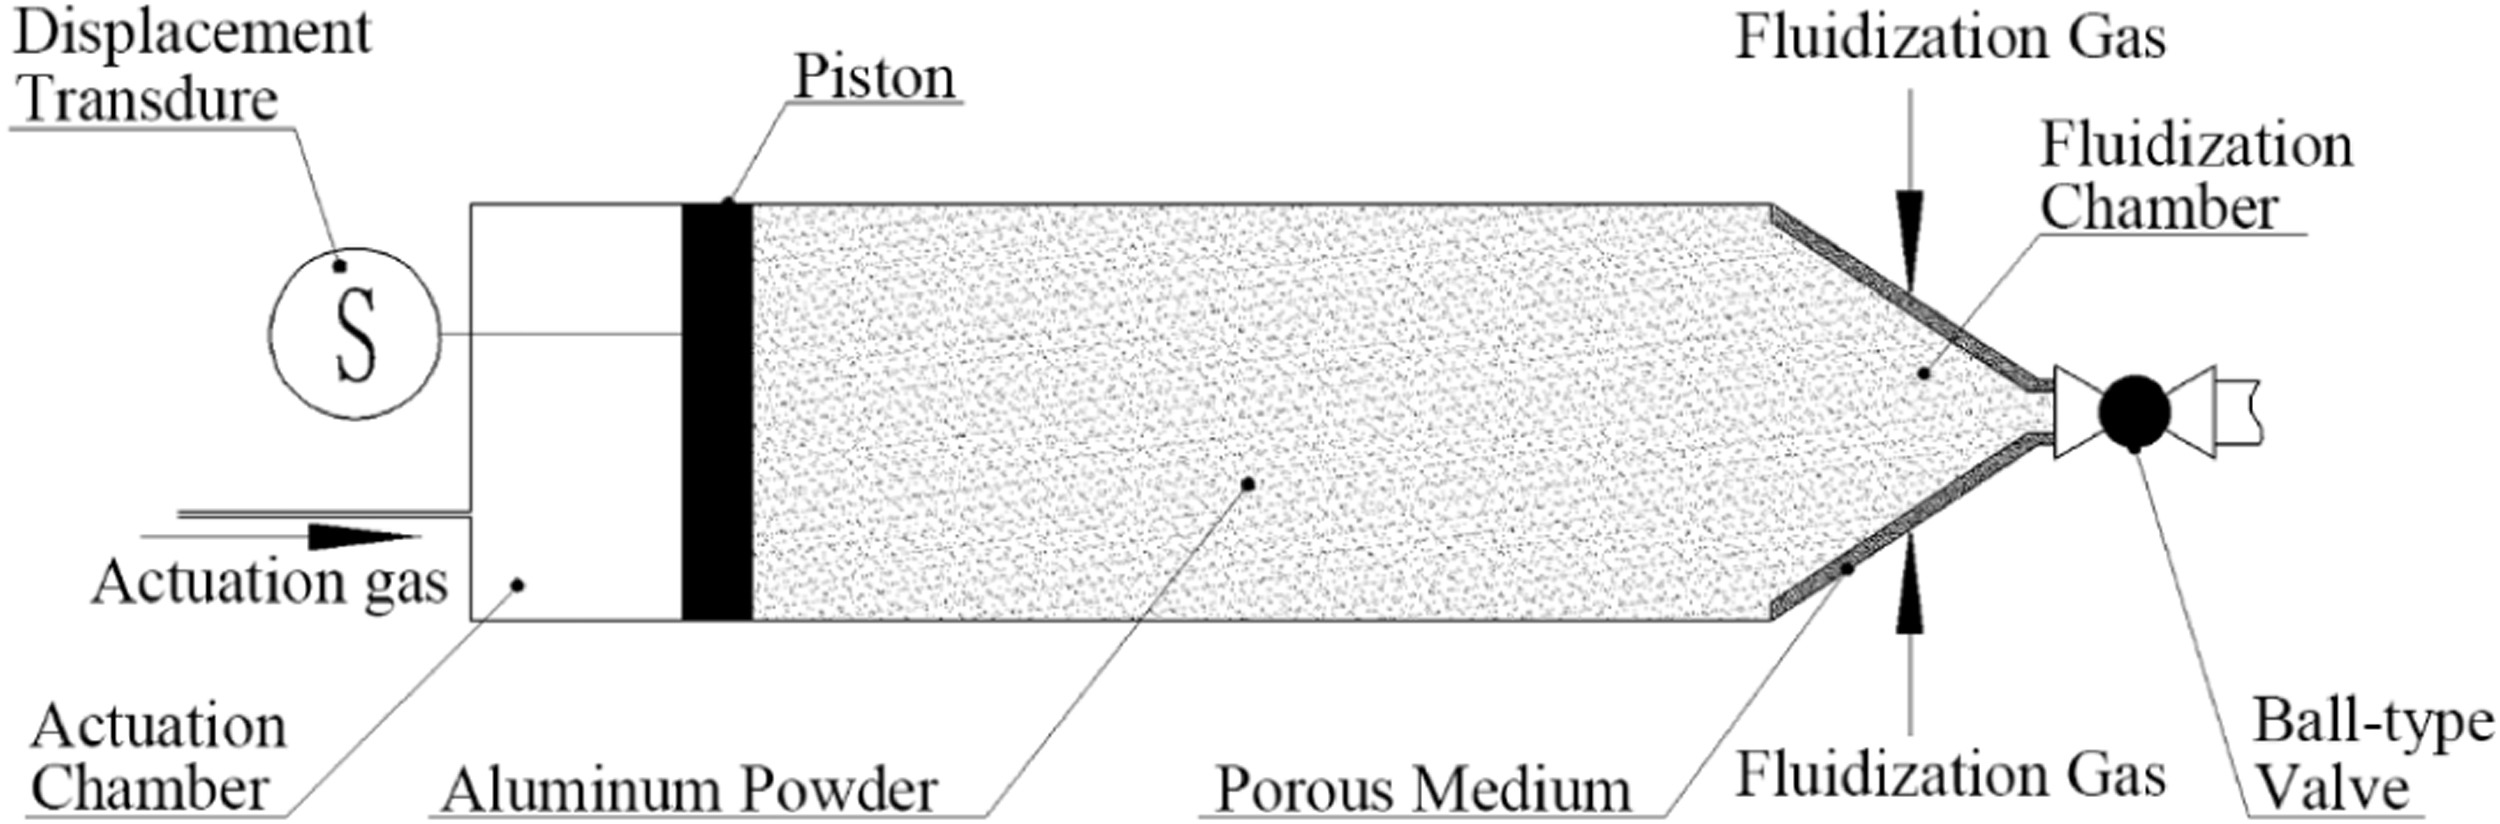
\includegraphics[width=\textwidth]{../report_assets/gas_driven.png}
        \caption*{Gas Driven Piston~\cite{Li2016}}
    \end{minipage}
    \caption{Examples of Gas and Motor Actuated Pistons from Literature}\label{fig:actuation-piston}
\end{figure}

The second innovation came in the form of fluidising the powder from the piston face as well as the end of the tank, seen in \autoref{fig:fluid-from-the-back}. It has been shown that fluidising further back in the tank leads to higher mass flow rates and a lower amount of powder left in the system~\cite{Tang22}. This means the feed systems fluidised at the inlet have a greater range of mass flow rates to operate in.
\begin{figure}[htbp]
    \centering
    
    \begin{minipage}{0.9\textwidth}
        \centering
        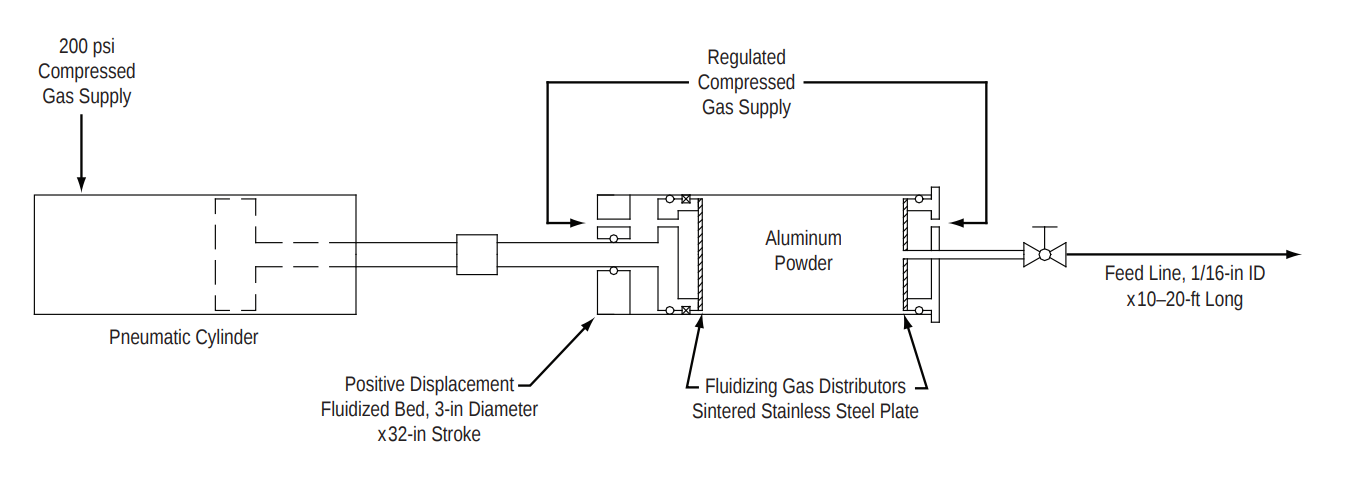
\includegraphics[width=\textwidth]{../report_assets/des_evo_3.png}
        \caption{Example of Fluidisation at the Inlet from Literature~\cite{NASA2008_20080002287}}\label{fig:fluid-from-the-back}
    \end{minipage}
   
\end{figure}

The final revision was removing the fluidisation at the end of the tank all together, seen in \autoref{fig:gas-permeable}. Having to design the tank outlet to have a porous medium in it's walls requires reinforcing the strength of the tank which adds mass to the design. The additional plumming to provide the outlet fluidising gas also adds additional mass that can be reduced by just fluidising from behind.
\begin{figure}[htbp]
    \centering
    
    \begin{minipage}{0.8\textwidth}
        \centering
        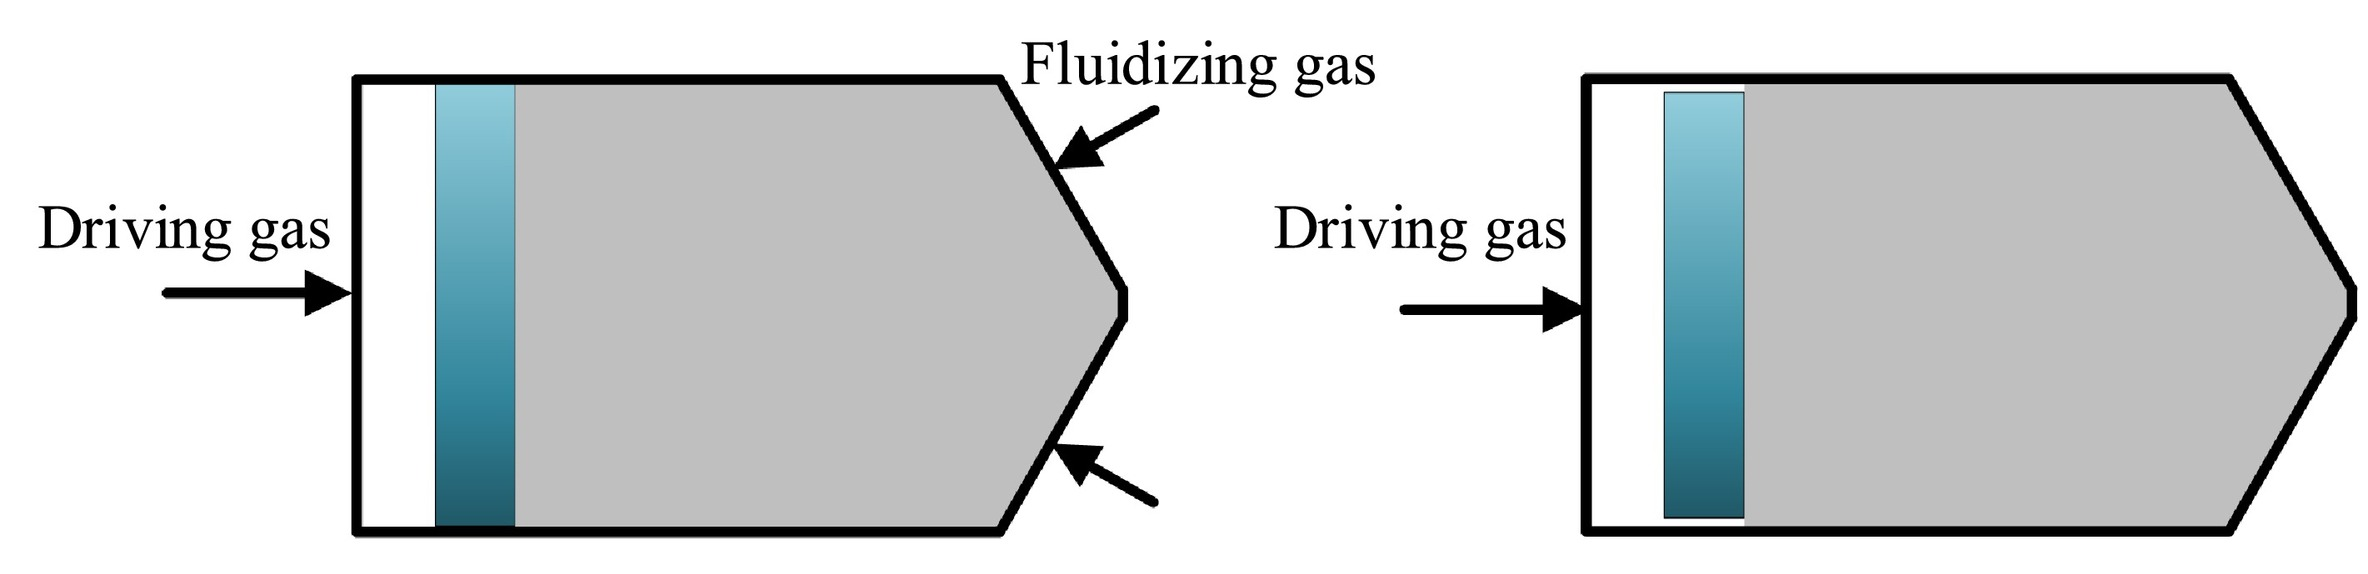
\includegraphics[width=\textwidth]{../report_assets/des_evo_1.png}
        \caption{Inlet Fluidised Design~\cite{TANG2023118406}}\label{fig:gas-permeable}
    \end{minipage}
   
\end{figure}

Powder feed systems for solid rocket motors have many similarities to CSAM feed systems but differ in one notable way. While the particles in cold spray are fed into atmospheric conditions, or vacuum conditions for space applications, the particles in an engine are fed into the high pressure combustion chamber. This means the downstream pressure for the two systems is very different and explains why the majority of the literature focuses on high pressure powder feed systems. Given that lower pressures, \>1MPa, are less extensively investigated, this report can add to the analysis of such conditions.
% A commonly cited first implementation of a fluisising powder feed system consists of a cylindrical tank with a piston to constrain the powder to the outlet~\cite{LI2021712}. As this paper is no longer in the public domain, the author assumes that the piston is motor actuated as the use of gas-actuated pistons is often credited to later work~\cite{TANG2023118406} and how the tank is fluidised is unknown. The gas actuated piston revisions pass the fluidising gas down the piston rod and through a gas-permeable piston face~\cite{Loftus1972}. Close to the outlet there is a porous section in which the fluidising gas is supplied. Despite the number of papers referencing this research, the author is unable to validate whether this is still in the public domain. This design was improved upon by pneumatically actuating the piston and supplying the fluidising gas through the piston shaft, with the gas exiting a porous plate mounted on the piston face~\cite{Loftus1972}. 

\section{Propellent Management Devices}
The need to store material in space is not new and has recieved extensive research, especially regarding the storage of propellants. Like the manufacturing system presented later, propulsion systems can be disturbed or damaged due to the contents of the tank not being constrained to the outlet~\cite{Hartwig2016}. Solutions to this problem already exist in the form of propellant management devices.
\begin{figure}[htbp]
    \centering
    
    \begin{minipage}{0.25\textwidth}
        \centering
        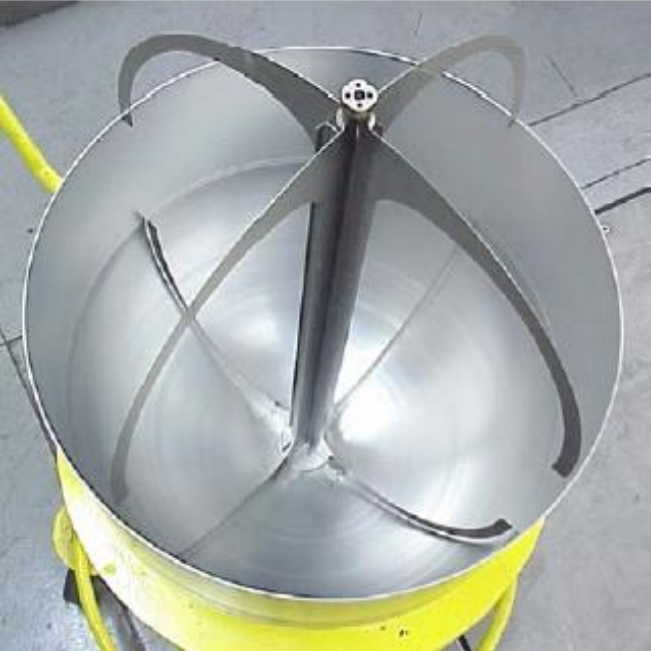
\includegraphics[width=\textwidth]{../report_assets/vane.png}
        \caption{Tank Vanes~\cite{Hartwig2016}}\label{fig:vane}
    \end{minipage}
    \hspace{3em}
    \begin{minipage}{0.47\textwidth}
        \centering
        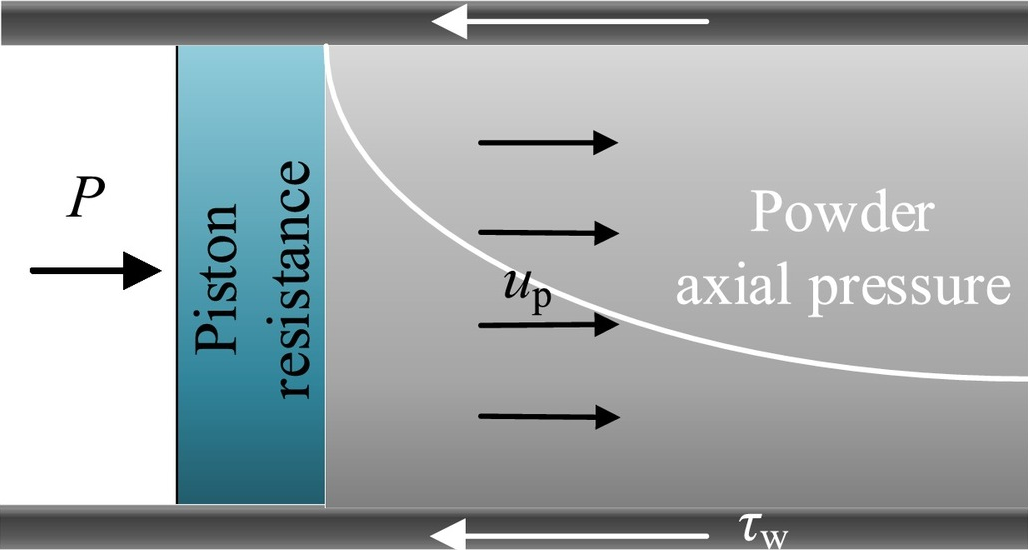
\includegraphics[width=\textwidth]{../report_assets/piston.png}
        \caption{Piston Tank Diagram~\cite{TANG2023118406}}\label{fig:piston}
    \end{minipage}
    
\end{figure}
Vanes, seen in \autoref{fig:vane}, sponges and galleries have been well tested in microgravity environments~\cite{Hartwig2016} but rely on surface tension so are only applicable to storing liquid. Positive expulsion devices like bladders, diaphragms and pistons, seen in \autoref{fig:piston}, mechanically force propellant towards the outlet and, therefore, are suitable for powder applications. 

Alongside allowing for more reliable powder dispension, constraining the powder can prevent problematic dynamics like sloshing from occuring in the tank reducing the systems footprint on the rest of the spacecraft and making attitude control easier.


% sloshing phenomenon, surface tension doesnt work, piston tanks and common issues.
% 1
% A Detailed Historical Review of Propellant Management
% Devices for Low Gravity Propellant Acquisition
% in jan folder
% given extra time come back to this and try and cite stuff about surface tension and cite maybe the rate of usage
\section{Management of Bulk Powder}\label{sec:bulk-powder}
Powder in a tightly-packed (bulk) form displays entirely different dynamics to that of powder in a fluidised state and is more complex to describe. This is because of the different types of forces between the particles~\cite{ZAFAR2017389}, contact points and the friction associated changing due to plastic and elastic deformation~\cite{TALEBI2024211} and the particles freedom to rearrange. 
\begin{figure}[htbp]
    \centering
    \begin{minipage}{0.5\textwidth}
        \centering
        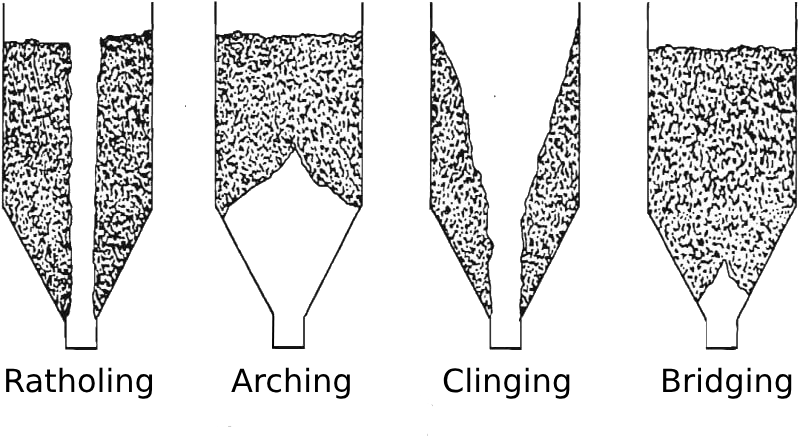
\includegraphics[width=\textwidth]{../report_assets/bridging.png}
        \caption{Common Powder Structures~\cite{911Metallurgist_binsflow}}\label{fig:bulk_powder_structures}
    \end{minipage}
\end{figure}
This means powders respond to stress somewhere between a fluid and a frictional solid: they dilate under shear, compact under normal load, and can sustain stable structures, seen in \autoref{fig:bulk_powder_structures}, that block flow in hoppers. 
\section{Modelling Two-phase flow}
Given that microgravity is very expensive to achieve experimentally, the project relies on correlating the simulated behaviour under gravity with the experiment and then comparing this with the simulated behaviour under microgravity. Therefore the method used for simulation is outlined below.

Because there are so many different kinds of two phase flow, there are countless ways to model the behaviour.  The general idea applies the conservation of mass, momentum and energy equations for both phases over a fixed control volume. While this formulation is sufficient to perform for direct numerical simulation of the flow, simplifying assumptions are often made to avoid the unrealisitic computational requirements~\cite{enwald1996eulerian}. Simulating fluidised beds is currently done through two main methods: the Eulerian-Lagrangian method and the Eulerian-Eulerian method~\cite{C6RA28615A}. The first regards the particles as a discrete phase and the fluidising gas as a continuum. It then tracks the dynamics of each particle in the Lagrangian reference frame and couples them to the continuum through interphase momentum exchange~\cite{SUBRAMANIAM2013215}. The second models both as fluids, tracking the amount of particle phase present in the mixture and uses constitutive equations of granular theory to couple the two continua~\cite{C6RA28615A}. As discussed in \autoref{sec:numerical-setup}, the Eulerian-Eulerian model is most applicable to the system so is further outlined.


While the drag model is not a constitutive equation in the strict sense, in Eulerian-Eulerian models, it acts like one and closes the system of equations. Therefore the choice of drag model greatly impacts the resulting dynamics, especially with respect to the behaviour of bubbles and bed expansion. The gidaspow model was found to be the most representative for fluidising beds~\cite{C6RA28615A}.

